\documentclass[12pt]{article}

\usepackage{graphicx}
\usepackage{caption}
\usepackage{amsmath, amssymb, amsthm}
\usepackage{booktabs}
\usepackage{enumitem}
\usepackage{geometry}
\geometry{margin=1in}
\usepackage{xcolor}
\usepackage{float}
% \usepackage[numbers,sort&compress]{natbib} % number style
\usepackage[colorlinks=true, allcolors=blue]{hyperref} %For hyperlinks, usually must be the last package called
\usepackage[capitalise]{cleveref} % must be loaded after hyperef
\usepackage{tabularx}
\usepackage{float}
\usepackage[normalem]{ulem} % normalem keeps \emph working normally




% Packages for algorithms and pseudocode
\usepackage{algorithm}
\usepackage{algpseudocode}

\title{NPSC3000 End of Year Report: Can Reinforcement Learning Outperform Traditional Methods for Cloud Resource Allocation}
\author{
\textbf{Student:} Ty Riekert \\
\textbf{Supervisor:} Elham Mardaneh \\
\textbf{Co-supervisor:} Tony Mathew
}
\date{Sept 2026}



\begin{document}
\maketitle
\begin{abstract}
    The problem of resource allocation (RA) is a critical issue amongst cloud providers \cite{saidi2023, sdn2021, vinothina2012, parikh2013, mohamaddiah2014}. There exists a shared set of physical resources such as servers, network, storage, and user applications that they need to manage in real-time. These resources are dynamically managed and allocated in the form of jobs to virtual machines (VMs), and it's a vital challenge to ensure operations, traffic performance, and energy conservation of these VMS are properly managed. One approach in which this can be modelled is as a Resource-Constrained Project Scheduling (RCS) optimisation problem. With user applications and jobs arriving in real-time, this problem is considered to be online in that the overall decision horizon for algorithms to assign jobs to machines is non-deterministic. Since cloud RA is also inherently a multi-objective and dynamic problem, traditional methods have been shown to struggle \cite{lbts2024, 10854610, DAHMANI2025100616, DBLP:journals/corr/abs-2107-04333}, however, recent studies highlight the strong potential of reinforcement learning (RL) in handling dynamic and large-scale environments reflected in such a problem \cite{saidi2023, autoscaling2023, lbts2024, dynamic2026}. Building on the insights of such papers, this report aims to implement a reinforcement learning agent that can outperform traditional methods on the comparison of tardiness, late and assigned jobs, and total objective reward. Versions and iterations of two RL approaches were implemented: proximal policy optimisation (PPO) and advantage actor critic (A2C) agents. Preliminary results on the offline scheduling case show PPO fails to learn useful assignments under every configuration tested (reward tuning, hyperparameter search, Lagrangian, and pointer-network architecture alike), converging to tardiness which is statistically indistinguishable from heuristics that ignore deadlines entirely. In contrast, A2C with potential-based reward shaping \cite{ng1999shaping} achieves results competitive with a few heuristic baselines on the fixed data instance setting, althought on a randomized set of instances, all RL models fail to obtain meaningful results. \textcolor{red}{In the online setting with stochastic job arrivals, the RL agent with action-space overhaulingly outperforms the majority of the heuristics in some architectures, with less than average in other iterations}. Fully closing the gap between RL and heuristic or rule-based policies is still under work.

\end{abstract}


\newpage
\section{Project Deliverables}
The aim of this project is to formulate cloud resource allocation as a mathematical optimisation and reinforcement learning problem. Implementing and rigorously evaluating RL models against established methods. The specific deliverables are:
\begin{itemize}
    \item Conduct comprehensive research on current findings and machine learning in cloud resource allocation
    \item Formulate a mathematical model of the cloud RA problem, expressed as a resource-constrained scheduling optimisation problem
    \item Create a corresponding Markov Decision Process (MDP) formulation of the reinforcement learning agent
    \item Implement the code of the scheduling environment
    \item Implement the code for the reinforcement learning agent(s)
    \item Evaluate the trained agents against classical scheduling heuristics to determine under what conditions reinforcement learning outperforms traditional methods.
\end{itemize}
The last item is not done with a single `train and compare' run, but is an iterative process repeated throughout the entire last half of the project. A constant loop of training, evaluating against baselines, examining and researching behaviour and faults, and revising.

\section{Background}
\subsection{Cloud Computing}
Cloud computing refers to the use of computing services and resources delivered over the internet, and resource allocation (RA) is one of the most critical challenges facing cloud providers today \cite{saidi2023, huawei2022}. As cloud infrastructure underpins the majority of modern computing services, effectively allocating physical resources, like compute or network bandwidth to a continuously arriving stream of workloads, has become of vital importance to providers \cite{sdn2021}. Poor allocation can lead to poor metrics in response time, environmental sustainability, energy or power efficiency, throughput, makespan, utilisation and more \cite{cloudkpi2010, dvbpp2026, mohamaddiah2014, anuradha2014}.


\subsubsection{Cloud RA}
Cloud RA can be decomposed into several coupled problems. Virtual machine (VM) placement takes the cloud provider's physical servers as virtual machines subject to resource constraints like CPU and memory. User requests are then assigned to those virtual machines. This is widely regarded as the core RA subproblem \cite{saidi2023}. Task scheduling divides the workload evenly across all available resources while minimising execution and response time \cite{lbts2024}. Autoscaling dynamically adjusts resource capacity to match fluctuating demand in real time \cite{autoscaling2023}, and load balancing distributes incoming tasks evenly to avoid hotspots \cite{lb2024}.
\newline
Solutions to these problems generally fall into three categories
\begin{itemize}
    \item \textbf{Exact Methods}. Algorithms that always solve a problem optimally
    \item \textbf{Approximation Methods}. These methods are used when exact algorithms become computationally infeasible. Two main classes are heuristics which algorithms design to quickly construct or improve a single solution, and metaheuristics that are more higher-level and guide heuristic methods in a strategic manner \cite{alkhalifa2025comparative}
    \item \textbf{Machine learning}. Algorithms that are based on enforcing a set of rules to get the machine to learn on data
\end{itemize}

Exact methods guarantee optimality on small instances, scale terribly, and are then only useful for lower bound estimates. Heuristics and metaheuristics scale well, but can yield approximate solution that may not be sufficiently accurate. Systematic reviews within this field identify four major problems of these approximation methods: scalability, adaptability, generalisation multi-objective complexity, high computational cost with scale, and real-time decision making \cite{mohamaddiah2014, lbts2024, 10854610, DAHMANI2025100616, ml_ra_litrev2025, hu2021attend2pack}.


\subsubsection{Motivations for Machine Learning}
The above mentioned limitations motivate a growing body of work of applying machine learning, and reinforcement learning specifically, to combinatorial and scheduling problems. A fixed heuristic relies on designer intuition to determine what makes a job important and applies that rule unchanged through deployment. RL still requires design choices such as what should it optimise for, but the policy on how to decide assignments of a job to a machine are learnt during training in an environment that should reflect the deployment environment \cite{ml_ra_litrev2025}. Systematic reviews of RL for scheduling or bin packing report encouraging growth in this area \cite{DAHMANI2025100616}, and prior systems like DeepRM \cite{mao2016deeprm} and Decima \cite{mao2019decima} showed learned schedulers matching or exceeding hand-designed rules on cluster workloads.
\newline
%              This project examines a policy-gradient \cite{chadia2023understandingRL, lehmann2024policygradients, sutton2000policy, vanheeswijk2021fourpolicies}, actor-critic RL methods; and Advantage Actor-Critic (A2C), the synchronous version of A3C \cite{schulman2017ppo, mnih2016a3c, apxml_a2c_a3c_2026, aigreeksActorCritic, chadia2023understandingRL, konda1999actorcritic}. We also examine variations like hyper-heuristics \cite{burke2013hyperheuristicsurvey, lassoued2026hyperheuristic, cie2025dispatchruleselection}, and hybrid RL \cite{min2022atctuning, chen2024drlgphh}. These learning algorithms are then placed against classical dispatching heuristics \cite{vepsalainen1987atc, ortools}.


This project examines two actor-critic RL methods; Proximal Policy Optimisation (PPO) and Advantage Actor-Critic (A2C), the synchronous version of A3C \cite{schulman2017ppo, mnih2016a3c, apxml_a2c_a3c_2026, aigreeksActorCritic, chadia2023understandingRL, konda1999actorcritic}. We also examine variations like hyper-heuristics \cite{burke2013hyperheuristicsurvey, lassoued2026hyperheuristic, cie2025dispatchruleselection}, and hybrid RL \cite{min2022atctuning, chen2024drlgphh}. These learning algorithms are then placed against classical dispatching heuristics \cite{vepsalainen1987atc, ortools}.
    

\subsubsection{Project Motivation}
RL for cloud RA is in active research \cite{ml_ra_litrev2025, DAHMANI2025100616}, but existing papers mainly review only a few objectives for RL, and compare against a limited set of baselines. Exploring a more multi-objective approach or modelling as a resource constrained optimisation (RCO) problem isn't as expressed in industry. Most papers use a bin-packing or VM placement approach, many explore improving resource usage of RL \cite{cloud_rco}, and so a more comprehensive review of RL in cloud RA is necessary. Through existing papers' research on problem decisions, structure, models, new algorithms or findings for using RL, we can implement a suite of approaches to truly see how well RL performs based on the research before us. 
\newline
We would like to see \textbf{under which objectives and conditions does RL outperform classical scheduling algorithms on the problem of cloud RA?}


\subsubsection{Markov Decision Process}\label{sec:MDP_ssSection}
The Markov Decision Process (MDP) is a foundational framework for decision making in stochastic and uncertain environments \cite{DRL_Intrusion}. It is the core structure used for an RL program. At any time $t$ it has a state $\mathcal{s}_t$ that reflects the current state of the environment, and the actions available $\mathcal{a}_t$ (often masked to get rid of infeasible actions \cite{huang2020invalidmasking}). The agent must go from state $\mathcal{s}_t$ to $\mathcal{s}_{t+1}$ by choosing an action $\mathcal{a}_t$. 
\newline

An MDP is described as a tuple $(S,A,P,R,\gamma)$. We have the sets $S$ (state space) and $A$ (action space). $P$ is the transition probability that satisfies the Markov property,
\begin{equation}\label{Markov_Property}
    p(s_{t+1}|s_1,a_1,s_2,a_2,\dots,s_t,a_t)=p(s_{t+1}|s_t,a_t)
\end{equation}

$p(s'|s,a)\in P$ describes the total probability of transferring to a specific state $s'$ by taking action $\mathcal{a}$ in the given state $\mathcal{s}$. The reward function $R:S\times A\rightarrow \mathbb{R}$ gives the expected immediate reward $R(s,a)=\mathbb{E}[r_t|s_t=s,a_t=a]$ that the agent receives after taking action $a$ in state $s$ - alternatively this can be defined as $r(s,a,s')\in\mathbb{R}$. Finally, $\gamma\in(0,1]$ is the discount factor that can be used to indicate short-term or long-term importance of rewards. The MDP loop can be seen in Figure \ref{fig:MDP_Diagram}. The final goal of an agent in MDP is to maximise the overall reward.
\begin{figure}
    \centering
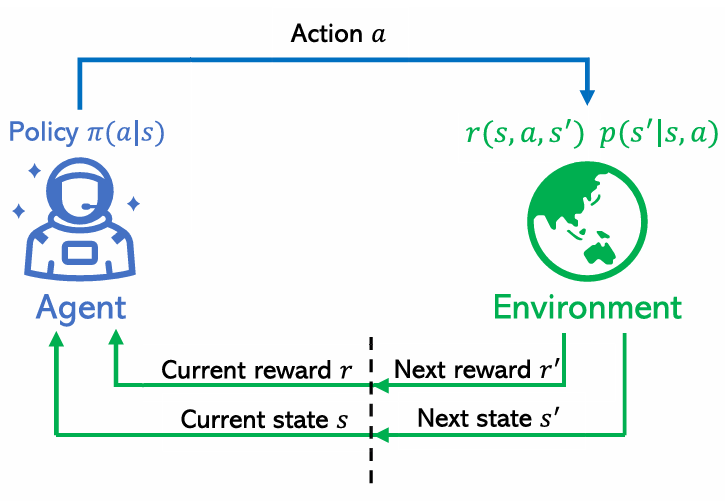
\includegraphics[width=0.5\linewidth]{Images/MDP_Diagram.png}
    \caption{Agent Interaction With MDP}
    \label{fig:MDP_Diagram}
\end{figure}

\subsection{Reinforcement Learning}
RL is a decision-making computer program that starts without any prior knowledge, by learning through its own experiences of repeated random interactions with an environment. It has the key benefit of being able to learn by exploring its training environment, and receiving feedback from this environment based on its actions \cite{LADOSZ20221}. After training, the agent is graded on its performance with a different environment and then deployed.
\newline

Fundamentally, an RL problem is formalised as a Markov Decision Process (MDP), as explained in Section~\ref{sec:MDP_ssSection} \cite{LADOSZ20221, DRL_Intrusion}. The goal of the agent is to maximise the expected total reward defined by its reward function, by learning a policy: a probability distribution over actions $a_t$ for a given state $s_t$ that makes the best decisions possible. RL methods fall into two main families. \textbf{Value-based} methods learn the expected return of each action and greedily choose the action with the highest estimate (typically), while \textbf{policy-gradient} methods directly adjust the policy's parameters towards higher return \cite{williams1992reinforce}. Hybrid methods such as \textbf{actor-critic} combine the two. A critic learns the expected return of each action, a value-based method, and an actor updates the policy using the critic's predictions, a policy-gradient method \cite{konda1999actorcritic}.

The final goal of the agent is to maximise the sum of the rewards given from the environment. It makes decisions with a policy, a function that takes in a state and outputs the best possible action. There are two types of RL, policy approximation and value approximation. Policy approximation directly updates the policy function's parameters to make the best decisions - having to gradient descent to every action. Value function approximation introduces a value function to predict the downstream rewards of an action to simplify the policy update. Finally, actor-critic combines the two.



\section{Methodology}
\subsection{Problem Formulation}
Consider the general problem we would like to research. There is some cloud computing environment that receives a set of jobs according to some distribution that need to be assigned to a set of physical machines. Each job $j$ has a fixed processing duration $p_j$, a fixed multi-dimensional vector of its resource requirements $a_{jr}$ (e.g CPU, memory) which it occupies for the entire duration of its processing, and a due date $d_j$ which the job should be completed by. Jobs are assumed to be independent of one another. To reflect that some jobs matter more than others, each job is given a priority weight $w_j$, which we can assume to be set externally according to some business needs.
\newline

Jobs are served by a set of identical machines, each limited only by a fixed capacity $C_r$. A machine may process several jobs simultaneously, provided the combined resource usage of every job does not exceed its capacity in any dimension. We model the scheduling to be non-preemptive: each job is assigned to exactly one machine at a single start time, and runs uninterrupted until completion. We discretise time into integer steps over a finite planning horizon $H$. The tardiness of a job $j$ is then,
\begin{equation}\label{eq:tardiness}
    T_j = \max\left(0,\; s_j + p_j - d_j\right).
\end{equation}
Notation is summarised in Appendix ~\ref{sec:AppendixA}, and the full constraint set in Appendix ~\ref{} \textcolor{red}{ADD REFERENCE TO CONSTRAINT APPENDIX}

\subsection{Objective Functions}
The objective functions are the functions we would like to optimise for. In this project, two objective functions were used. The first (v1) weighs machine count (with machine activation $y_m$), weighted tardiness ($w_jT_j$) and peak utilisation $\theta$ with objective weights $\lambda$:
\begin{equation}\label{eq: Initial Objective Function}
      \min \; \lambda_1 \sum_{m \in M} y_m \;+\; \lambda_2 \sum_{j \in J}
  w_j T_j \;+\; \lambda_3\, \theta,
  \end{equation}
Experiments under v1 revealed that the training reward was inefficient with reward hacking \cite{skalse2022rewardhacking}, and that unscheduled jobs incurred no loss. Essentially the objective could be optimised without considering tardiness. Moreover, the machine activation and hotspot penalties were found to be weak in that the activation penalty was an unnecessary once-off penalty, and the hotspot term inadvertently went against energy metrics and provides no real help to the RL agents. This term also opposes energy-efficient consolidation \cite{energyaware2012, fan2007powerprovisioning}. The revised objective (v2) is a sum of multiple metrics each weighted by $\lambda$:
\begin{equation}\label{eq:objective-v2}
    \min \; J = \lambda_S \sum_{j} w_j T_j^{2}
              + \lambda_U \sum_{j} w_j U_j + \lambda_E E,
\end{equation}
In order it covers squared tardiness ($w_j T_j^{2}$), weighted late job count ($w_jU_j$), and energy usage ($E)$. With this new objective, we can control which metrics we would like to examine for the project (by changing their weighted significance). Squared tardiness was included to incentivize choosing to have many slightly late jobs over having a few extremely late jobs. It also discourages never assigning a job, which v1 struggled with.

\subsection{Offline and Online Cases}
We would like to study two cases of the problem: offline when all jobs are known and available at $t=0$ but only a single job can be assigned at each time index, and an online case where jobs arrive (revealed) over time through a Poisson process \cite{kleinrock1975queueing, mao2016deeprm} but multiple jobs can be assigned at any given timestep. 
\newline
The difficulty for the online case of the random job arrivals is set by the load factor
\begin{equation}\label{eq:rho}
    \rho = \max_{r \in R} \frac{\nu\, \mathbb{E}[p_j a_{jr}]}{|M|\, C_r},
\end{equation}
where $\nu$ is the arrival rate. Work accumulates when $\rho\ge1$. Loads from $\rho = 0.50$ to $1.10$ are studied, with log-normal job sizes matching the right-skewed distributions of real cluster traces \cite{reiss2012googletrace, cortez2017resourcecentral}.


\subsection{Markov Decision Process}
To formulate this problem for our algorithms, we use a Markov Decision Process $(S,A,P,R,\gamma)$ as discussed in section ~\ref{sec:MDP_ssSection}.
\newline

\paragraph{State $S$}. We define the state to hold each currently waiting job's ($j\in J_t\subseteq J$) features $F_j=(p_j, A_j, d_j, w_j)$, along with each currently processing job where a job enters the processing set $P_t\subseteq J$ when it gets assigned. For each processing job, we instead hold $G_j=(m_j,s_j,p_j)$ that includes which machine the job is assigned to, its start time and total duration. On top of the jobs, we include include the remaining capacity of each machine,
\begin{equation}\label{eq:remaining-capacity}
    R_{mrt} = C_r - \sum_{j \in P_t:\ m_j = m} a_{jr},
\end{equation}
and $y=(y_m)_{m\in M}$ to record which machines are online. This yields a state vector,
\begin{equation}\label{eq:state}
    s_t = \big(J_t,\ P_t,\ \{F_j\}_{j \in J_t},\ \{G_j\}_{j \in P_t},\ \{R_{mrt}\}_{m \in M,\, r \in R},\ y,\ t\big).
\end{equation}
\paragraph{Action Space $A$}. At each step, the agent can take actions of assigning waiting jobs to machines, and/or idling,
\begin{equation}\label{eq:action-flat}
    \mathcal{A}_t = \{(j, m) : j \in J_t,\ m \in M\} \cup \{\text{idle}\}.
\end{equation}
For the offline case, an agent can only produce a single action at each time step. For the online case, an agent can continuously do actions at the same step $t$, only progressing to the next time step when it decides to idle. 

\paragraph{Transition dynamics $P$.} Briefly, an assignment action $(j, m)$ moves job $j$ from $J_t$ to $P_t$ with $s_j = t$ and $m_j = m$, activating machine $m$ if needed. When time advances (after every action for offline, and only after idle for online), completed jobs leave the processing set by \cref{eq:processing-update}, their capacity is released, and online, newly arrived jobs join $J_{t+1}$. Transitions are deterministic for offline and stochastic for online only through arrivals.
\begin{equation}\label{eq:processing-update}
    P_{t+1} = \{k \in P_t : s_k + p_k > t + 1\},
\end{equation}

\paragraph{Reward $R$.} This project used both v1 and v2 rewards where stated in later sections (\cref{sec:objectives}).







\subsection{Methods Compared - ADD REFERENCES FOR EACH ALGORITHM}
In this project, a variety of algorithms are examined, grouped into four categories. We summarise these algorithms as follows. 

\subsubsection{Learning Algorithms}
\paragraph{Reinforcement Learning.} All RL policy methods examined are actor-critic methods: A2C and PPO for their robustness and simplicity. We consider these algorithms under several action-space designs:
\begin{itemize}
    \item \textbf{Option 0 -- Direct Job-Machine Selection:} The policy picks a (job, machine) pair with a flat network or pointer-network architecture \cite{vinyals2015pointernet, kool2019attention}. A large discrete action space is a known struggle with policy-gradient methods.
    \item \textbf{Option 1 -- Hyper-heuristic Rule Selection:} The policy chooses which dispatching rule to apply at each decision \cite{burke2013hyperheuristicsurvey, lassoued2026hyperheuristic}
    \item \textbf{Option 2 -- Priority Learning:} The policy scores jobs directly with either learned or directly engineered features, a hybrid of RL.
    \item \textbf{Option 3 -- Windowed Priority:} Option 2, but masked to only the 20 most urgent jobs \cite{mao2016deeprm}
    \item \textbf{Option 4 -- Action Branching:} Job and machine are chosen by two separate heads instead of together (flat) \cite{tavakoli2018actionbranching}
\end{itemize}
Moreover, variants of the two RL algorithms: Reward Constrained Policy Optimisation (RCPO) for a different reward function approach, and PPO-Lagrangian were also examined.

\subsubsection{Baseline Algorithms}
\paragraph{Dispatching Heuristics}. Each heuristic combines a priority rule to choose the next job, and a placement rule to choose the next machine.
\begin{itemize}
    \item \textbf{Priority Rules:} Earliest Deadline First (EDF) and Least Slack Time (LST), which prioritise urgency; Shortest and Longest Processing Time (SPT) and (LPT); Weighted SPT (WSPT); First-Come-First-Served (FCFS), and the Apparent Tardiness Cost (ATC) rule, balancing job weight, length and urgency.
    \item \textbf{Placement Rules:} First-Fit, Best-Fit, Worst-Fit, and Consolidate, a more energy aware approach \cite{energyaware2012}
    \item \textbf{Tetris:} A multi-resource packing heuristic scoring job-machine pairs jointly.
\end{itemize}

\paragraph{Metaheuristic:}
\begin{itemize}
    \item \textbf{Particle Swarm Optimisation (PSO)}. Each particle encodes a job and machine ordering which is decoded with a placement rule into a schedule. 
\end{itemize}

\paragraph{Exact Solver:}
\begin{itemize}
    \item \textbf{CP-SAT}. Constraint programming which models the scheduling problem and environment exactly, finding the proven optimum schedule if given enough time, otherwise a lower bound on the optimum.
\end{itemize}


\subsection{Implementation}
The environment, agents and evaluation pipeline are implemented in Python\footnote{\url{https://github.com/Ethan-Ty-Riekert/Neural-Knapsack-Research-Project}} using Gymnasium and Stable-Baselines3 \cite{raffin2021sb3}. The original environment and mathematical formulation implementation into code was done manually, with all model implementations, training and evaluation done with Claude Code (Anthropic) to allow for fast code iteration and implementation.
\begin{itemize}
    \item \textbf{Context. }Claude is provided with the latest version of the current research report, formulations, and experimental logs
    \item \textbf{Rules. }A fixed set of rules for Claude to follow: Every design decision has to be cited and justified, or derived. Implementation, research and discussions have to remain mathematical grounded
    \item \textbf{Benchmarking and Results. }All results and benchmarks are run autonomously by Claude with a constant queue, ready for personal review.
    \item \textbf{Diagnostics and Research. }Unexpected results and failures are investigated and checked against literature
    \item \textbf{Recording and Revisions. }Every decision and result is to be recorded in an experiment log
\end{itemize}
All modeling decisions and formulations are reviewed and approved personally. Using Claude as a coding assistant allowed for far more experiments to be run and analysed, along with constant model improvements and iterations than would otherwise have been possible independently. It also allowed for easier discussions of modelling decisions against other papers. Moreover, weekly optimisation, mathematical rigour, and factual scans were done with separate Claude agents to ensure correctness.




\subsubsection{Experimental Setup}
\paragraph{Offline} instances have 100 jobs, 10 machines, 4 resources with $C_r=30$, $H=100$. Job durations and demands are drawn uniformly from $\{1,\dots,9\}$, and job weights $\{1,\dots,5\}$, with deadlines of medium tightness ($\mathrm{TF} = 0.5$) \cite{potts1985wtardiness}. A matching preset with all $w_j = 1$ is generated to isolate the effects of considering weights.

\paragraph{Online} instances use the same setup with addition of Poisson arrivals over $[0, H)$ at loads $\rho\in\{0.50, 0.75, 0.95, 1.10\}$ and deadline slack drawn between 10 and 60. Moreover job resource sizes are log-normal, mean-matched to the offline distribution.

\paragraph{Training}. An agent learns by interacting with an environment over a sequence of episodes. One episode is one complete problem instance, i.e an instance of making decisions until the horizon $H$ is reached for some given environment. Every episode uses a newly generated random instance of job parameters so that the agent never sees the same problem twice and can thereby generalise. Every RL action design was trained with PPO and A2C, with the same tuning and training budgets. Hyperparameters were tuned with Optuna \cite{akiba2019optuna} using the TPE sampler \cite{bergstra2011tpe} and median pruning. 20 trials of 100,000 steps for each model design, algorithm and case (offline and online) were put into the Optuna search. Every 25,000 steps, each trial was evaluated against 5 validation instances and stopped early if it was worse than the median of earlier trials. The best configuration of hyperparameters is then trained for 300,000 steps across 4 parallel environments. Because RL deviates between training runs, each best configuration was trained individually 3 times on different random seeds, and final results are reported as the mean and standard deviation across these runs.



\paragraph{Testing and Evaluation}. Every method - RL and heuristic included - is evaluated on the same 50 test instances which have not been seen in training or tuning. We report the mean and standard deviation of the objective function over these test instances, along with any other metrics we would like to examine such as quality of assigning, wait time, maximum tardiness, and mean waiting time - despite not being optimized for.

\section{Results}
Please review the github \href{https://github.com/Ethan-Ty-Riekert/Neural-Knapsack-Research-Project/tree/main/Results}{results page} for all obtained results.
\subsection{Initial Formulation (v1)}
\subsubsection{Offline}
The interactive results page can be seen \href{https://htmlpreview.github.io/?https://github.com/Ethan-Ty-Riekert/Neural-Knapsack-Research-Project/blob/main/Results/v1_legacy_reward/ALL_RESULTS_2026-07-24_to_2026-09-22/scheduler_results_atlas.html}{here}, the main findings are expressed below.
\\
Importantly, the v1 objective did not capture scheduling quality as intended, meaning that the raw reward signal alone is not a reliable indicator of performance. On reward, the RL methods A2C and PPO matched or beat the highest-reward heuristic, LPT+FirstFit (\cref{fig:v1-reward}). On tardiness, however, no correctly functioning RL method beat the best heuristic, LST, and all of them also scheduled fewer jobs and had more late jobs than LST (\cref{fig:v1-tard,fig:v1-sched,fig:v1-late}). The top five methods on reward, tardiness, jobs scheduled and late jobs are shown in \cref{fig:v1-reward,fig:v1-tard,fig:v1-sched,fig:v1-late}. Note that these results are for the constant weight scenario. The uniform weight distribution was only introduced late into v1 and no RL method could beat heuristics.

\begin{figure}[htbp]
\centering
\includegraphics[width=0.85\linewidth]{Images/v1_off_c_50_reward_top5.png}
\caption{Top five methods by v1 reward on 50 held-out offline instances (higher is better). The two highest-reward methods both have very high tardiness, showing that the v1 reward did
not measure scheduling quality.}
\label{fig:v1-reward}
\end{figure}

\begin{figure}[htbp]
\centering
\includegraphics[width=0.85\linewidth]{Images/v1_off_c_50_tard_top5.png}
\caption{Top five methods by mean total tardiness under v1 (lower is better). The only method below LST achieves it by abandoning about 45\% of the jobs.}
\label{fig:v1-tard}
\end{figure}

\begin{figure}[htbp]
\centering
\includegraphics[width=0.85\linewidth]{Images/v1_off_c_50_sched_top5.png}
\caption{Top five methods by mean number of jobs scheduled, out of 100, under v1 (higher is better). Scheduling nearly every job does not imply they all met
deadlines.}
\label{fig:v1-sched}
\end{figure}

\begin{figure}[htbp]
\centering
\includegraphics[width=0.85\linewidth]{Images/v1_off_c_50_late_top5.png}
\caption{Top five methods by mean number of late jobs, out of 100, under v1 (lower is better).}
\label{fig:v1-late}
\end{figure}

\subsubsection{Online}
Similar graphs for the online case are seen in stated github link. In summary, job arrival load $\rho \approx 0.75$ was examined with no RL method outperforming the best heuristic in either constant weights or uniform weight distribution.


\subsection{Revised Formulation (v2)}


\section{Discussion}


\section{Conclusion}

\section{Future Work}
\begin{itemize}
    \item More research and consideration into the online case. The online case remains incredibly complex and this project only touches on it briefly.
    \item Look more into hybrid architectures \cite{ml_ra_litrev2025}
    \item Adopt simulation-based training and interactive learning environments \cite{ml_ra_litrev2025}
    \item Considering more and different metrics and objectives
    \item Examine the large action-space failure of policy-based methods, and evaluate how different methods compare and potentially aid in this project's future findings. This includes replacing the current pointer network encoding with graph neural networks for job/machine encoding \cite{gnn2024jsspsurvey}, and a variety of action-space reductions and branching \cite{tavakoli2018actionbranching}
    \item Evaluate large discrete action space methods such as the Wolpertinger architecture \cite{dulacarnold2015largeactionspaces}
    \item Investigate more improvements to many models like RCPO, ATC dispatching, rule-selection and other algorithms implemented
    \item Evaluate the trained policies against real-world data from e.g Google cluster trace or Microsoft Azure trace
    \item Conduct a formulation and environmental review of problem structure for different goals. Many small changes can be made that may increase performance
\end{itemize}



\newpage
\section{Marking Outline}
Your task is to:
\newline
Write a report of approximately 3000 – 5000 words (excluding gures, captions, references, tables, and appendices) that details your activities through this unit. The content and layout of your report will depend on the type of project/s you undertook as part of this unit. A combination of visual and textual information should be included in the report. The format of reports may vary across discipline areas. While each report will be unique in terms of focus and outcomes, the following sections should be included:


\begin{itemize}
    \item A succinct title that reects the focus of the project
    \item Your name, your supervisor’s name(s)
    \item Concise introduction to your project which orientates the reader (Abstract)
    \item Project aims/goals/objectives
    \item Specific project outputs/deliverables
    \item Background : reference to literature justifying the value and importance of the project
    \item Methodology
    \item Results: Present results in a format relevant to your discipline. Use graphical and tabular format where appropriate.
    \item Discussion – what you achieved/discovered, the relevance of what you achieved
    \item Conclusion
    \item Future projects that may build on this project or new ideas for future projects emerging from your work this year
\end{itemize}



Not included in the word count, but must be included:

Data Management Plan -- access to raw data, processed data, code repository
GenAI use statement - declare use of any GenAI software and how it was used.
References
\newpage
%\nocite{*}
\bibliographystyle{IEEEtran}
% \bibliographystyle{IEEEtranSN}
\bibliography{references}




\newpage
\section{Appendix}



\subsection{Appendix A}\label{sec:AppendixA}
\begin{table}[htbp]
\centering
\caption{Nomenclature}
\label{tab:nomenclature}
\begin{tabular}{ll}
\hline
\multicolumn{2}{l}{\textbf{Sets}}\\
\hline
$J$ & Set of jobs, indexed by $j$ \\
$P$ & Set of processing jobs \\
$J_t$ & Jobs currently waiting (not yet started) at time $t$ \\
$M$ & Set of candidate machines, indexed by $m$ \\
$R$ & Set of resource types, indexed by $r$ \\
$\mathcal{T}$ & Set of discrete time periods, indexed by $t$ \\
\hline
\multicolumn{2}{l}{\textbf{Parameters}}\\
\hline
$p_j$ & Processing duration of job $j$ \\
$a_{jr}$ & Requirement of job $j$ for resource type $r$ \\
$C_r$ & Capacity of each machine for resource type $r$ \\
$H$ & Length of the planning horizon \\
$d_j$ & Due date or deadline of job $j$ \\
$w_j$ & Priority weight or penalty weight of job $j$ \\
$\tau_j$ & Arrival time of job $j$ (for offline is $0$) \\
$\nu$, $\rho$ & Arrival rate and load factor for online jobs \\
$\lambda_1,\lambda_2,\lambda_3$ & Weights in the v1 objective \\
$\lambda_S,\lambda_T,\lambda_U,\lambda_E$ & Weights in the v2 objective \\
\hline
\multicolumn{2}{l}{\textbf{Decision variables}}\\
\hline
$x_{jmt}$ & 1 if job $j$ starts on machine $m$ at time $t$; 0 otherwise \\
$y_m$ & 1 if machine $m$ is used; 0 otherwise \\
$s_j$ & Start time of job $j$ \\
$T_j$ & Tardiness of job $j$ \\
$U_{mrt}$ & Total usage of resource $r$ on machine $m$ at time $t$ \\
$\theta$ & Maximum utilisation ratio over all machines, resources, and time periods \\
\hline
\end{tabular}
\end{table}

\subsection{Appendix B}\label{sec:AppendixB}


\end{document}

